% MidlineSparseMoE-GP: full pipeline with diagrams and derivations
% Upload this single file to Overleaf (TeX Live 2022+). Compile with pdfLaTeX.
\documentclass[11pt,a4paper]{article}

\usepackage[margin=1in]{geometry}
\usepackage{amsmath,amssymb,amsthm,bm}
\usepackage{mathtools}
\usepackage{booktabs}
\usepackage{enumitem}
\usepackage{hyperref}
\usepackage{xcolor}
\usepackage{tikz}
\usetikzlibrary{arrows.meta,positioning,fit,calc,shapes.geometric,decorations.pathreplacing}
\usepackage{algorithm}
\usepackage{algpseudocode}
\usepackage{microtype}

\hypersetup{colorlinks=true,linkcolor=blue!50!black,citecolor=blue!50!black,urlcolor=blue!60!black}

\title{\textbf{MidlineSparseMoE-GP}:\\
Pipeline, Diagrams, and Derivations}
\author{Implementation notes matching \texttt{gpplus/models/midline\_sparse\_moe.py}\\
(SpectralGPPlus / experiments\_MOEGP)}
\date{\today}

\newcommand{\R}{\mathbb{R}}
\newcommand{\E}{\mathbb{E}}
\newcommand{\Ncal}{\mathcal{N}}
\newcommand{\softplus}{\operatorname{softplus}}
\newcommand{\sigmoid}{\sigma}
\newcommand{\Keff}{K_{\mathrm{eff}}}
\newcommand{\Khat}{K_{\mathrm{hat}}}
\newcommand{\Kmodes}{K_{\mathrm{modes}}}
\newcommand{\Kmax}{K_{\max}}

\begin{document}
\maketitle

\begin{abstract}
MidlineSparseMoE-GP is a two-stage model for \emph{co-located} multimodal regression:
modes of \(p(y\mid x)\) that are \emph{not} a function of \(x\) (so input-dependent
MoE gating is misspecified). Stage~1 fits a single \textbf{exact} Gaussian process (GP)
midline \((\mu_0,\sigma_0)\) on the full training set. Stage~2 learns an overcomplete
mixture of additive offsets with Hard-Concrete sparsity, mixture weights, and a
multiplicative variance carve-out of \(\sigma_0^2\). Training maximizes mixture
likelihood plus geometric / sparsity regularizers. Evaluation dual-reports expert
activity \((\Keff,\Khat)\) versus peaks of the predictive density \((\Kmodes)\).
This document derives every quantity as implemented.
\end{abstract}

\tableofcontents
\newpage

%==============================================================================
\section{Problem setting}
%==============================================================================

\subsection{Co-located multimodality}
Data \(\{(x_i,y_i)\}_{i=1}^n\) with \(x_i\in\R^{d}\) (typically \(d{=}1\) in probes)
and scalar \(y_i\). The conditional \(p(y\mid x)\) may be multimodal even when
\emph{mode identity does not depend on \(x\)}:
\begin{equation}
  p(y\mid x)
  =
  \sum_{m=1}^{M^\star}
  \pi_m^\star\,
  \Ncal\!\bigl(y;\, f_m^\star(x),\, (\sigma_m^\star)^2\bigr),
  \qquad
  \text{with gates not encoding ``which mode'' via \(x\).}
\end{equation}
\textbf{A01} (bimodal, equal \(\sigma\)) and \textbf{A04} (trimodal, unequal \(\sigma\))
are co-located probes. \textbf{A02} (step discontinuity) is \emph{separated}:
regimes \emph{do} depend on \(x\); MidlineSparse is not designed for that case.

\subsection{What ``sparse'' means here}
``Sparse'' refers to \textbf{Hard-Concrete expert switches} \(\alpha_k\in[0,1]\),
not sparse/inducing-point GPs and not per-expert data partitions.
Stage~1 uses one exact GP on the \emph{entire} training domain.

\begin{figure}[ht]
\centering
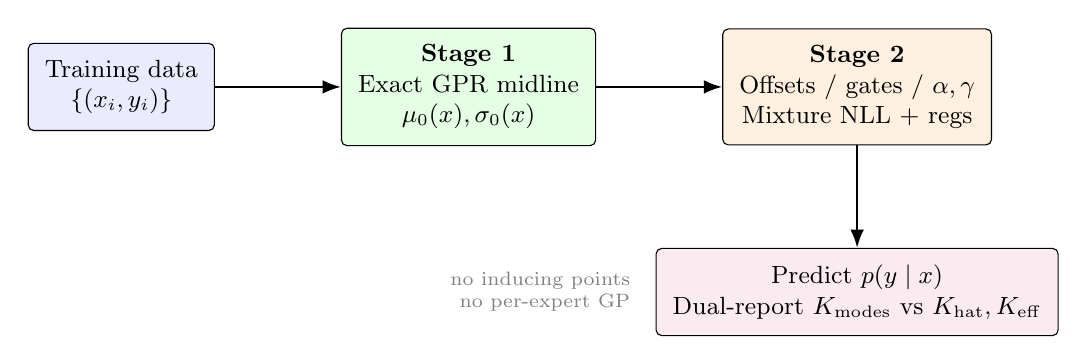
\begin{tikzpicture}[
  box/.style={draw,rounded corners=2pt,align=center,inner sep=6pt,font=\small},
  arr/.style={-{Latex},thick}
]
\node[box,fill=blue!8] (data) {Training data\\ \(\{(x_i,y_i)\}\)};
\node[box,fill=green!10,right=1.6cm of data] (s1) {\textbf{Stage 1}\\ Exact GPR midline\\ \(\mu_0(x),\sigma_0(x)\)};
\node[box,fill=orange!12,right=1.6cm of s1] (s2) {\textbf{Stage 2}\\ Offsets / gates / \(\alpha,\gamma\)\\ Mixture NLL + regs};
\node[box,fill=purple!8,below=1.3cm of s2] (pred) {Predict \(p(y\mid x)\)\\ Dual-report \(\Kmodes\) vs \(\Khat,\Keff\)};
\draw[arr] (data) -- (s1);
\draw[arr] (s1) -- (s2);
\draw[arr] (s2) -- (pred);
\node[left=0.2cm of pred,align=right,font=\scriptsize,text=gray] {no inducing points\\ no per-expert GP};
\end{tikzpicture}
\caption{High-level two-stage pipeline.}
\label{fig:pipeline}
\end{figure}

%==============================================================================
\section{Stage 1: exact GP midline}
%==============================================================================

\subsection{Model}
Fit a single exact GP regression on all \(n\) points:
\begin{equation}
  y(x)
  =
  f_0(x) + \varepsilon,
  \qquad
  f_0\sim\mathcal{GP}\bigl(m(\cdot),\, k(\cdot,\cdot)\bigr).
\end{equation}
Implementation uses constant mean, RBF-style kernel (\texttt{LogScaleKernel(GaussianKernel)}),
and \texttt{LogGaussianLikelihood}. Training: multi-init L-BFGS via \texttt{GPTrainer}.

After fitting, evaluate the posterior predictive on the training inputs:
\begin{align}
  \mu_0(x_i)
  &=
  \E[f_0(x_i)\mid \mathcal{D}],
  \\
  \sigma_0(x_i)
  &=
  \sqrt{\mathrm{Var}[y(x_i)\mid \mathcal{D}]},
\end{align}
stored as buffers \(\_mu0\_train\), \(\_std0\_train\).

\subsection{Capped Stage-2 ceiling (optional)}
Residual scale
\begin{equation}
  \hat s
  =
  \mathrm{Std}\bigl(y_i-\mu_0(x_i)\bigr).
\end{equation}
With fraction \(c=\texttt{std0\_cap\_frac}\) (default \(0.3\)):
\begin{equation}
  \sigma_0^{\mathrm{cap}}(x_i)
  =
  \min\bigl(\sigma_0(x_i),\, \max(c\,\hat s,\, 0.05)\bigr).
\end{equation}
If \texttt{use\_full\_gp\_variance=True} (legacy), Stage~2 uses \(\sigma_0\);
if \texttt{False} (champion \textbf{p12}), Stage~2 uses \(\sigma_0^{\mathrm{cap}}\).
Denote the chosen ceiling by \(\sigma_0^{\mathrm{mix}}(x)\).

\subsection{Offset seeding}
Residuals \(r_i=y_i-\mu_0(x_i)\). Seed \(K_{\max}\) offset biases from residual quantiles
(e.g.\ \(0.25\) and \(0.75\), then extra quantiles), centered to mean zero, written into
constant \(\delta\) or the MLP last-layer bias.

%==============================================================================
\section{Stage 2: MidlineSparse mixture}
%==============================================================================

Let \(\Kmax\) be the overcomplete expert budget (e.g.\ \(6\)).

\subsection{Parameters}
\begin{center}
\begin{tabular}{@{}llp{6.2cm}@{}}
\toprule
Symbol & Range & Role \\
\midrule
\(\alpha_k\) & \([0,1]\) & Hard-Concrete on/off for expert \(k\) \\
\(\pi_k(x)\) & simplex & Mixture / gate weight \\
\(\delta_k(x)\) & \(\R\) & Offset (constant or MLP) \\
\(\gamma_k\) & \((0,1)\) & Variance carve-out fraction \\
\bottomrule
\end{tabular}
\end{center}

\begin{figure}[ht]
\centering
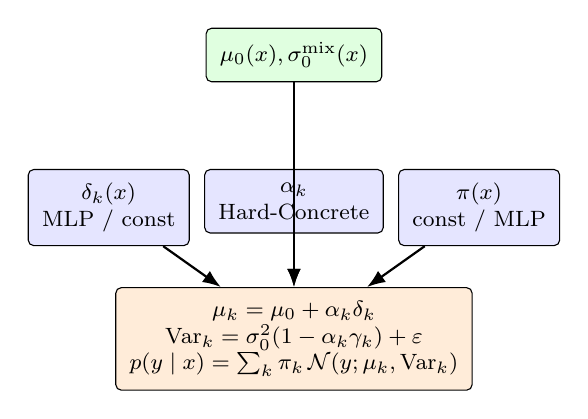
\begin{tikzpicture}[
  box/.style={draw,rounded corners=2pt,align=center,inner sep=5pt,font=\footnotesize},
  arr/.style={-{Latex},thick}
]
\node[box,fill=green!12] (mu0) {\(\mu_0(x),\sigma_0^{\mathrm{mix}}(x)\)};
\node[box,fill=blue!10,below left=1.1cm and 0.2cm of mu0] (delta) {\(\delta_k(x)\)\\ MLP / const};
\node[box,fill=blue!10,below=1.1cm of mu0] (alpha) {\(\alpha_k\)\\ Hard-Concrete};
\node[box,fill=blue!10,below right=1.1cm and 0.2cm of mu0] (pi) {\(\pi(x)\)\\ const / MLP};
\node[box,fill=orange!15,below=2.6cm of mu0] (mix) {
  \(\mu_k=\mu_0+\alpha_k\delta_k\)\\
  \(\mathrm{Var}_k=\sigma_0^{2}(1-\alpha_k\gamma_k)+\varepsilon\)\\
  \(p(y\mid x)=\sum_k \pi_k\,\Ncal(y;\mu_k,\mathrm{Var}_k)\)
};
\draw[arr] (mu0) -- (mix);
\draw[arr] (delta) -- (mix);
\draw[arr] (alpha) -- (mix);
\draw[arr] (pi) -- (mix);
\end{tikzpicture}
\caption{Stage~2 generative structure at a fixed \(x\).}
\label{fig:stage2}
\end{figure}

\subsection{Hard-Concrete gate \(\alpha_k\) (Louizos et al.)}
Let \(\log\alpha_k\) be unconstrained. Stretch constants
\((\gamma_{\mathrm{HC}},\zeta_{\mathrm{HC}})=(-0.1,1.1)\) and temperature
\(\beta_{\mathrm{HC}}=2/3\) (code names: \texttt{gamma}, \texttt{zeta}, \texttt{beta}
on \texttt{HardConcreteGate} --- \(\beta_{\mathrm{HC}}\) is \emph{not} an expert variance scale).

\paragraph{Deterministic (eval / reporting).}
\begin{equation}
  \alpha_k
  =
  \mathrm{clip}_{[0,1]}
  \Bigl(
    \sigmoid(\log\alpha_k)\,(\zeta_{\mathrm{HC}}-\gamma_{\mathrm{HC}})
    +
    \gamma_{\mathrm{HC}}
  \Bigr).
\end{equation}

\paragraph{Stochastic (training).}
Sample \(u\sim\mathrm{Unif}(0,1)\),
\begin{equation}
  s
  =
  \sigmoid\!\Bigl(
    \frac{\log u - \log(1-u) + \log\alpha_k}{\beta_{\mathrm{HC}}}
  \Bigr),
  \qquad
  \alpha_k=\mathrm{clip}_{[0,1]}\bigl(s(\zeta_{\mathrm{HC}}-\gamma_{\mathrm{HC}})+\gamma_{\mathrm{HC}}\bigr).
\end{equation}

\paragraph{Complexity (L0 surrogate).}
With threshold \(t=-\gamma_{\mathrm{HC}}/\zeta_{\mathrm{HC}}\),
\begin{equation}
  \mathcal{L}_{\mathrm{HC}}
  =
  \sum_{k=1}^{\Kmax}
  \sigmoid\!\bigl(
    \log\alpha_k
    -
    \beta_{\mathrm{HC}}\log t
  \bigr).
\end{equation}

\subsection{Gates \(\pi(x)\)}
\texttt{ConstantGate}: logits \(\to\) temperature-softmax \(\pi\in\Delta^{\Kmax-1}\)
(independent of \(x\)).
\texttt{GatingNetwork}: MLP \(\to\) softmax (used on A02 probes).

\subsection{Offsets and pinning}
Raw offsets \(\delta_k^{\mathrm{raw}}(x)\) from a constant vector or MLP.
Pin so the gated mean offset has zero\(\pi\alpha\)-weighted center:
\begin{equation}
  w_{ik}
  \propto
  \pi_k(x_i)\,\alpha_k,
  \qquad
  \delta_{ik}
  =
  \delta_{ik}^{\mathrm{raw}}
  -
  \sum_{j} w_{ij}\,\delta_{ij}^{\mathrm{raw}}.
\end{equation}
Expert means:
\begin{equation}
  \boxed{
  \mu_k(x)
  =
  \mu_0(x)
  +
  \alpha_k\,\delta_k(x).
  }
\end{equation}

\subsection{Variance carve-out}
\begin{equation}
  \boxed{
  \mathrm{Var}_k(x)
  =
  \bigl[\sigma_0^{\mathrm{mix}}(x)\bigr]^2
  \,(1-\alpha_k\gamma_k)
  +
  \varepsilon,
  }
  \qquad
  \gamma_k=\sigmoid(\texttt{raw\_gamma}_k).
\end{equation}
Active experts with \(\gamma_k\to 1\) \emph{carve} variance below the GP ceiling;
\(\gamma_k\to 0\) keeps a fat blob (mode-merging risk on A04).

\paragraph{Historical note (free expert scale \(\beta_k\)).}
An optional multiplier \(\beta_k\ge 1\) was explored
(\(\mathrm{Var}_k\leftarrow\mathrm{Var}_k\cdot\beta_k\) with
\(\beta_k=1+\softplus(\texttt{raw\_beta}_k)\)) to allow unequal widths above
\(\sigma_0^2\). On A04 it was \textbf{inert} (\(\beta\approx 1\) even with
\(\lambda_\beta=0\)); NLL does not push free scale when the GP ceiling is already
large. Production / champion settings mute it (\(\beta_k\equiv 1\),
\texttt{free\_expert\_scale=False}). Recovery relies on capped \(\sigma_0\),
\(\gamma\) priors, and the recovery margin---not \(\beta\).

%==============================================================================
\section{Mixture likelihood}
%==============================================================================

For observation \(i\),
\begin{equation}
  p(y_i\mid x_i)
  =
  \sum_{k=1}^{\Kmax}
  \pi_k(x_i)\,
  \Ncal\!\bigl(y_i;\,\mu_k(x_i),\,\mathrm{Var}_k(x_i)\bigr).
\end{equation}
Negative log-likelihood (batch mean):
\begin{equation}
  \boxed{
  \mathrm{NLL}
  =
  -
  \frac{1}{n}
  \sum_{i=1}^{n}
  \log\sum_{k=1}^{\Kmax}
  \exp\!\Bigl(
    \log\pi_k(x_i)
    +
    \log\Ncal(y_i;\mu_k,\mathrm{Var}_k)
  \Bigr).
  }
\end{equation}
Implementation uses \texttt{logsumexp} over experts (stable).
\textbf{No mixture-mean MSE} is used (would collapse co-located modes toward \(\mu_0\)).

%==============================================================================
\section{Usage, separation, and dual counts}
%==============================================================================

\subsection{Soft usage (Option E)}
Average gate mass \(\bar\pi_k=n^{-1}\sum_i\pi_k(x_i)\) (or \(\pi_k\) if constant).
With thresholds \((\varepsilon,\tau)=(\texttt{keff\_eps},\texttt{keff\_tau})\):
\begin{equation}
  \tilde\alpha_k
  =
  \sigmoid\!\Bigl(
    \frac{\alpha_k\bar\pi_k - \varepsilon}{\tau}
  \Bigr).
\end{equation}

\subsection{Separation scores}
For pinned curves \(\delta_{\cdot k}\),
\begin{equation}
  d_k
  =
  \min_{j\neq k}
  \frac{1}{n}\sum_i \lvert\delta_{ik}-\delta_{ij}\rvert,
  \qquad
  s_k
  =
  \tanh(d_k / L),
\end{equation}
with \(L=\texttt{sep\_length}\). Near-duplicate experts get \(s_k\approx 0\).

\subsection{Effective / hard expert counts}
\begin{align}
  \boxed{
  \Keff
  =
  \sum_{k=1}^{\Kmax}
  \tilde\alpha_k\, s_k
  },
  \qquad
  \boxed{
  \Khat
  =
  \#\{k:\, \alpha_k\bar\pi_k \ge \varepsilon\}.
  }
\end{align}
\(\Keff\) can exceed \(1\) when multiple distinct used slots are active.
Stage~2 sparsifies \(\sum_k\tilde\alpha_k\), \emph{not} \(\softplus(\Keff-1)\)
(which would punish a correct multimodal count).

\begin{figure}[ht]
\centering
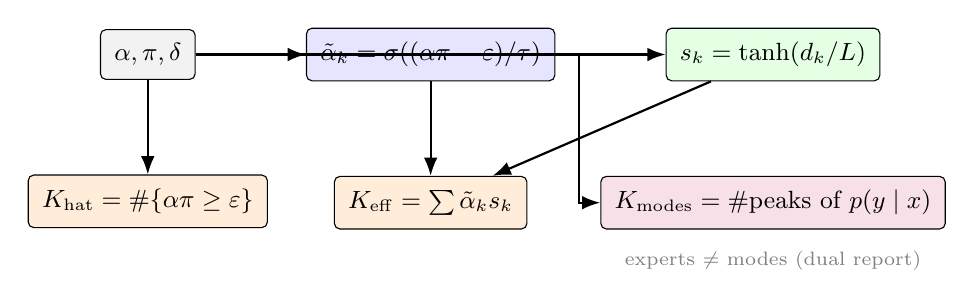
\begin{tikzpicture}[
  box/.style={draw,rounded corners=2pt,align=center,inner sep=5pt,font=\small},
  arr/.style={-{Latex},thick}
]
\node[box,fill=gray!10] (a) {\(\alpha,\pi,\delta\)};
\node[box,right=1.4cm of a,fill=blue!10] (u) {\(\tilde\alpha_k=\sigmoid((\alpha\pi-\varepsilon)/\tau)\)};
\node[box,right=1.4cm of u,fill=green!10] (s) {\(s_k=\tanh(d_k/L)\)};
\node[box,below=1.2cm of u,fill=orange!15] (ke) {\(\Keff=\sum\tilde\alpha_k s_k\)};
\node[box,below=1.2cm of a,fill=orange!15] (kh) {\(\Khat=\#\{\alpha\pi\ge\varepsilon\}\)};
\node[box,below=1.2cm of s,fill=purple!12] (km) {\(\Kmodes=\#\)peaks of \(p(y\mid x)\)};
\draw[arr] (a) -- (u);
\draw[arr] (a) -- (s);
\draw[arr] (u) -- (ke);
\draw[arr] (s) -- (ke);
\draw[arr] (a) -- (kh);
\draw[arr] (u.east) -- ++(0.3,0) |- (km);
\node[below=0.15cm of km,font=\scriptsize,text=gray]
  {experts \(\neq\) modes (dual report)};
\end{tikzpicture}
\caption{Dual reporting: expert slots vs density modes.}
\label{fig:dual}
\end{figure}

%==============================================================================
\section{Stage-2 loss (full derivation)}
%==============================================================================

Let \(\lambda_k(t)\) be the (possibly annealed) usage weight at Adam step \(t\).
If \(\lambda_k^{\mathrm{start}}\) is set,
\begin{equation}
  \lambda_k(t)
  =
  \lambda_k^{\mathrm{start}}
  +
  \frac{t-1}{T-1}
  \bigl(\lambda_k-\lambda_k^{\mathrm{start}}\bigr),
  \qquad t=1,\ldots,T
\end{equation}
(P4: form modes before sparsity prunes). Else \(\lambda_k(t)\equiv\lambda_k\).

\subsection{Regularizers}
\paragraph{Usage L0.}
\(
  \mathcal{L}_{\mathrm{usage}}
  =
  \sum_k \tilde\alpha_k.
\)

\paragraph{Separation.}
\(
  \mathcal{L}_{\mathrm{sep}}
  =
  \sum_{i<j}
  \tilde\alpha_i\tilde\alpha_j\,
  \softplus\!\bigl(m_{\mathrm{sep}}-\tfrac{1}{n}\sum_\ell\lvert\delta_{\ell i}-\delta_{\ell j}\rvert\bigr).
\)

\paragraph{Orphan / dead-mass (bidirectional \(\pi\)--\(\alpha\)).}
\begin{equation}
  \mathcal{L}_{\mathrm{orphan}}
  =
  \sum_k
  \Bigl[
    \alpha_k\,\softplus(\varepsilon-\bar\pi_k)
    +
    \bar\pi_k\,\softplus(\varepsilon-\alpha_k)
  \Bigr].
\end{equation}

\paragraph{Alive floor.}
\(
  \mathcal{L}_{\mathrm{alive}}
  =
  \softplus\!\bigl(0.8-\sum_k\tilde\alpha_k\bigr)
\)
(weight \(0.5\) in code).

\paragraph{Overlap (standardized mean gap).}
With \(\bar\mu_k,\bar\sigma_k\) averages over training rows,
\begin{equation}
  \mathrm{gap}_{ij}
  =
  \frac{\lvert\bar\mu_i-\bar\mu_j\rvert}{\bar\sigma_i+\bar\sigma_j},
  \qquad
  \mathcal{L}_{\mathrm{ov}}
  =
  \sum_{i<j}
  \tilde\alpha_i\tilde\alpha_j\,
  \softplus(m_{\mathrm{ov}}-\mathrm{gap}_{ij}).
\end{equation}

\paragraph{\(\delta\) L2.}
\(\mathcal{L}_{\delta}=\mathrm{mean}(\delta^2)\).

\paragraph{\(\gamma\) carve-out prior (p12 lever).}
\(
  \mathcal{L}_{\gamma}
  =
  \sum_k \tilde\alpha_k\,(1-\gamma_k)^2.
\)

\subsection{Total objective}
\begin{equation}
\boxed{
\begin{aligned}
  \mathcal{L}
  &=
  \mathrm{NLL}
  +
  \lambda_k(t)\,\mathcal{L}_{\mathrm{usage}}
  +
  \lambda_{\mathrm{sep}}\,\mathcal{L}_{\mathrm{sep}}
  +
  \lambda_{\alpha}\,\mathcal{L}_{\mathrm{HC}}
  +
  \lambda_{\mathrm{orphan}}\,\mathcal{L}_{\mathrm{orphan}}
  +
  0.5\,\mathcal{L}_{\mathrm{alive}}
  \\
  &\quad
  +
  \lambda_{\mathrm{ov}}\,\mathcal{L}_{\mathrm{ov}}
  +
  \lambda_{\delta}\,\mathcal{L}_{\delta}
  +
  \lambda_{\gamma}\,\mathcal{L}_{\gamma}
  +
  \lambda_{\mathrm{rec}}\,\mathcal{L}_{\mathrm{rec}}
  \;+\;
  \text{(optional mode-peak term)}.
\end{aligned}
}
\end{equation}
Optimized with Adam on \(\{\log\alpha,\texttt{raw\_gamma},\text{gate},\delta/\text{MLP}\}\).
The Stage~1 GP is \textbf{frozen}.

\begin{algorithm}[ht]
\caption{MidlineSparseMoE-GP training}
\begin{algorithmic}[1]
\State Fit exact GPR on \((X,y)\); store \(\mu_0,\sigma_0\) (and optional cap)
\State Seed \(\delta\) biases from residual quantiles
\For{\(t=1\) to \(T\)}
  \State Sample \(\alpha\) (stochastic HC); compute \(\pi(x),\delta(x),\gamma\)
  \State Form \(\mu_k,\mathrm{Var}_k\); compute \(\mathrm{NLL}\) and regularizers
  \State Adam step on Stage~2 parameters
\EndFor
\State Eval: deterministic \(\alpha\); report \(\Kmodes,\Khat,\Keff\), test NLL
\end{algorithmic}
\end{algorithm}

%==============================================================================
\section{Mode counting \(\Kmodes\)}
%==============================================================================

At probe \(x_\star\), form the mixture density on a \(y\)-grid:
\begin{equation}
  p(y\mid x_\star)
  =
  \sum_k
  \pi_k(x_\star)\,
  \Ncal\!\bigl(y;\,\mu_k(x_\star),\,\mathrm{Var}_k(x_\star)\bigr).
\end{equation}
\(\Kmodes(x_\star)\) = number of local maxima of \(p(\cdot\mid x_\star)\) above
\(0.05\cdot\max p\), with minimum separation \(5\%\) of the \(y\)-range
(\texttt{count\_density\_peaks}). Aggregate \(\Kmodes\) over probes as mean / round.
This is the \textbf{scientific target} for co-located claims; \(\Khat\) is diagnostic.

Optional training regularizer (generally \textbf{not} used for A04 fat-blob):
soft peak count on a coarse grid, then \(\softplus(\widehat K_{\mathrm{soft}}-2)\).

%==============================================================================
\section{Champion configuration (p12) and probes}
%==============================================================================

Noise-alleviation ablations identified \textbf{p12} = capped \(\sigma_0\) + \(\gamma\) prior:

\begin{center}
\begin{tabular}{@{}ll@{}}
\toprule
Knob & Champion p12 \\
\midrule
\texttt{use\_full\_gp\_variance} & \texttt{False} (use \(\sigma_0^{\mathrm{cap}}\)) \\
\(\lambda_{\gamma}\) & \(0.1\); init \(\texttt{raw\_gamma}\approx 2.2\) (\(\gamma\approx 0.9\)) \\
\(\lambda_{\mathrm{orphan}},\lambda_{\delta}\) & \(0.25,\ 0.02\) \\
\(\lambda_k,\lambda_k^{\mathrm{start}}\) & \(0.02,\ 0\to 0.02\) anneal \\
\(\lambda_{\mathrm{sep}},\lambda_{\mathrm{ov}}\) & \(0.1,\ 0.08\) \\
\texttt{free\_expert\_scale} & \texttt{False} (\(\beta\) muted; see historical note) \\
\bottomrule
\end{tabular}
\end{center}

Limitation stress (5 seeds): p12 recovers A01 and improves A04
(\(\Kmodes\approx 2.2\) vs true \(3\)); unimodal stays \(\approx 1\);
\textbf{A02 step fails} for both champion and classic (needs \(x\)-localized experts).

\begin{figure}[ht]
\centering
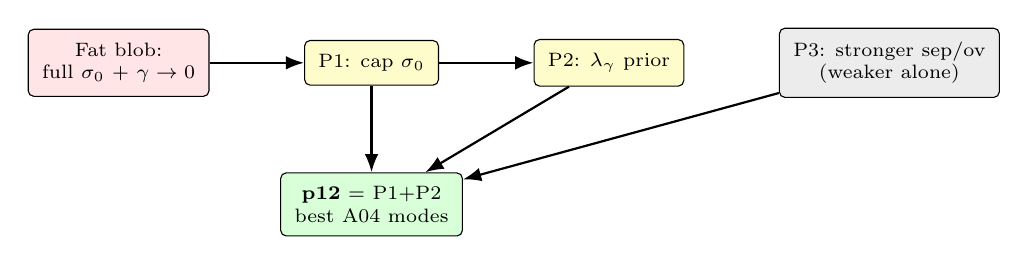
\begin{tikzpicture}[
  box/.style={draw,rounded corners=2pt,align=center,inner sep=5pt,font=\scriptsize},
  arr/.style={-{Latex},thick}
]
\node[box,fill=red!10] (fat) {Fat blob:\\ full \(\sigma_0\) + \(\gamma\to 0\)};
\node[box,fill=yellow!20,right=1.2cm of fat] (p1) {P1: cap \(\sigma_0\)};
\node[box,fill=yellow!20,right=1.2cm of p1] (p2) {P2: \(\lambda_\gamma\) prior};
\node[box,fill=green!15,below=1.1cm of p1] (p12) {\textbf{p12} = P1+P2\\ best A04 modes};
\node[box,fill=gray!15,right=1.2cm of p2] (p3) {P3: stronger sep/ov\\ (weaker alone)};
\draw[arr] (fat) -- (p1);
\draw[arr] (p1) -- (p2);
\draw[arr] (p1) -- (p12);
\draw[arr] (p2) -- (p12);
\draw[arr] (p3) -- (p12);
\end{tikzpicture}
\caption{Anti fat-blob levers; champion is P1+P2.}
\label{fig:p12}
\end{figure}

%==============================================================================
\section{Predictive equations (inference)}
%==============================================================================

At test \(x_\star\):
\begin{enumerate}[leftmargin=*]
  \item Posterior GP predictive \((\mu_0(x_\star),\sigma_0(x_\star))\); if capped mode,
        clamp \(\sigma_0\leftarrow\min(\sigma_0,\max_i\sigma_0^{\mathrm{cap}}(x_i))\).
  \item Deterministic \(\alpha_k\); \(\pi(x_\star)\); pinned \(\delta(x_\star)\); \(\gamma\).
  \item \(\mu_k,\mathrm{Var}_k\) as above.
  \item Mixture mean / variance:
  \begin{align}
    m(x_\star)
    &=
    \sum_k \pi_k\mu_k,
    \\
    v(x_\star)
    &=
    \sum_k \pi_k\bigl(\mathrm{Var}_k+\mu_k^2\bigr)
    -
    m(x_\star)^2.
  \end{align}
\end{enumerate}

%==============================================================================
\section{Recovery theory (modes of \(p(y\mid x)\))}
%==============================================================================

\subsection{Reduction to a 1D Gaussian mixture}
At a fixed probe \(x_\star\), MidlineSparse predicts
\begin{equation}
  p(y\mid x_\star)
  =
  \sum_{k=1}^{\Kmax}
  \pi_k\,
  \Ncal\!\bigl(
    y;\,
    \mu_0(x_\star)+\alpha_k\delta_k(x_\star),\,
    [\sigma_0^{\mathrm{mix}}(x_\star)]^2(1-\alpha_k\gamma_k)+\varepsilon
  \bigr).
\end{equation}
Active slots \(\mathcal A=\{k:\alpha_k\bar\pi_k\ge\varepsilon\}\).
Mode-recovery statements concern this finite univariate mixture, not the GP path \(x\mapsto\mu_0(x)\).

\subsection{Classical facts (not claimed as new)}
\begin{itemize}[leftmargin=*]
  \item \textbf{1D mode bound.} A \(k\)-component univariate Gaussian mixture has at most
        \(k\) modes (Carreira-Perpi\~{n}\'{a}n \& Williams; scale-space / Gaussian blurring).
  \item \textbf{Equal-\(\sigma\) bimodality.} For weights \(1/2\) and common variance \(\sigma^2\),
        two components are unimodal iff \(|\mu_1-\mu_2|\le 2\sigma\) (Eisenberger);
        Behboodian: \(|\mu_1-\mu_2|\le 2\min(\sigma_i,\sigma_j)\) is a sufficient unimodality
        condition. Thus modes appear only when means separate relative to noise scale.
  \item \textbf{A04 implication.} With unequal \(\sigma\in\{0.8,2,4\}\), a wide arm can
        swallow a narrow one: \(\Kmodes<M^\star\) is mathematically expected unless means
        separate relative to the \emph{largest} nearby \(\sigma\).
  \item \textbf{Parameters \(\neq\) modes.} GMM parameters can be identifiable under overlap
        (method of moments / ``disentangling Gaussians'') even when \(\Kmodes=1\).
        Component recovery does \emph{not} imply mode recovery.
\end{itemize}

\subsection{Conjecture template (assumptions; fit step unproven)}
\begin{quote}
\emph{Conjecture.}
If at \(x_\star\) the true mixture has \(M^\star\) components with
\[
  \min_{i\neq j}
  \frac{|\mu_i^\star-\mu_j^\star|}{\sigma_i^\star+\sigma_j^\star}
  \ge c
\]
for fixed \(c\ge 1\) (Behboodian-scale \(c=1\)), comparable weights, and Stage~2 returns
active components that \(L^2\)-match the truth up to label permutation within tolerance
\(\eta\), then \(\Kmodes(x_\star)=M^\star\).
\end{quote}
\noindent
MidlineSparse currently has \textbf{no proof} of the ``returns matching components'' step.
Algorithmic enforcement (\(\lambda_{\mathrm{rec}}\), capped \(\sigma_0\), \(\gamma\) prior,
separated init) aims to keep the fitted mixture inside the multimodal regime empirically.
A post-fit \emph{recovery certificate} checks standardized gaps \(g_{ij}\) on the fitted
model; it does not certify correctness versus the ground truth.

\subsection{Recovery regularizer}
Standardized gap on training averages \(\bar\mu_k,\bar\sigma_k\):
\begin{equation}
  g_{ij}
  =
  \frac{|\bar\mu_i-\bar\mu_j|}{\bar\sigma_i+\bar\sigma_j},
  \qquad
  \mathcal{L}_{\mathrm{rec}}
  =
  \sum_{i<j}
  \tilde\alpha_i\tilde\alpha_j\,
  \softplus(m_{\mathrm{rec}}-g_{ij}),
\end{equation}
with default \(m_{\mathrm{rec}}=1\) (Behboodian-scale). Weight \(\lambda_{\mathrm{rec}}\)
(default \(0\); recovery probes use \(0.15\)).

%==============================================================================
\section{Complexity and limitations}
%==============================================================================

\begin{itemize}[leftmargin=*]
  \item Stage~1 exact GP: \(\mathcal{O}(n^3)\) once; no inducing points.
  \item Stage~2: \(\mathcal{O}(T\cdot n\cdot \Kmax)\) (plus small \(\Kmax^2\) penalties).
  \item Strengths: co-located A01; partial A04 with p12; dual modes vs experts.
  \item Weaknesses: A02 separated regimes; A04 still short of \(K{=}3\); single shared
        GP midline cannot localize discontinuities the way classical MoE-GP partitions do.
\end{itemize}

%==============================================================================
\section{Notation cheat sheet}
%==============================================================================

\begin{center}
\begin{tabular}{@{}ll@{}}
\toprule
Symbol & Meaning \\
\midrule
\(\mu_0,\sigma_0\) & Stage~1 GP midline mean / predictive std \\
\(\sigma_0^{\mathrm{mix}}\) & \(\sigma_0\) or capped \(\sigma_0^{\mathrm{cap}}\) \\
\(\alpha_k\) & Hard-Concrete switch \\
\(\pi_k\) & Mixture weight \\
\(\delta_k\) & Additive offset (pinned) \\
\(\gamma_k\) & Carve-out fraction of \(\sigma_0^2\) \\
\(\tilde\alpha_k\) & Soft usage \\
\(s_k\) & Separation score \\
\(\Keff,\Khat\) & Soft / hard expert counts \\
\(\Kmodes\) & Peaks of \(p(y\mid x)\) \\
\bottomrule
\end{tabular}
\end{center}

\vspace{1em}
\noindent\textit{Code:}
\texttt{gpplus/models/midline\_sparse\_moe.py},
\texttt{experiments\_MOEGP/feasibility\_mode\_count/}.

\end{document}
